\begin{figure}
    \begin{center}
    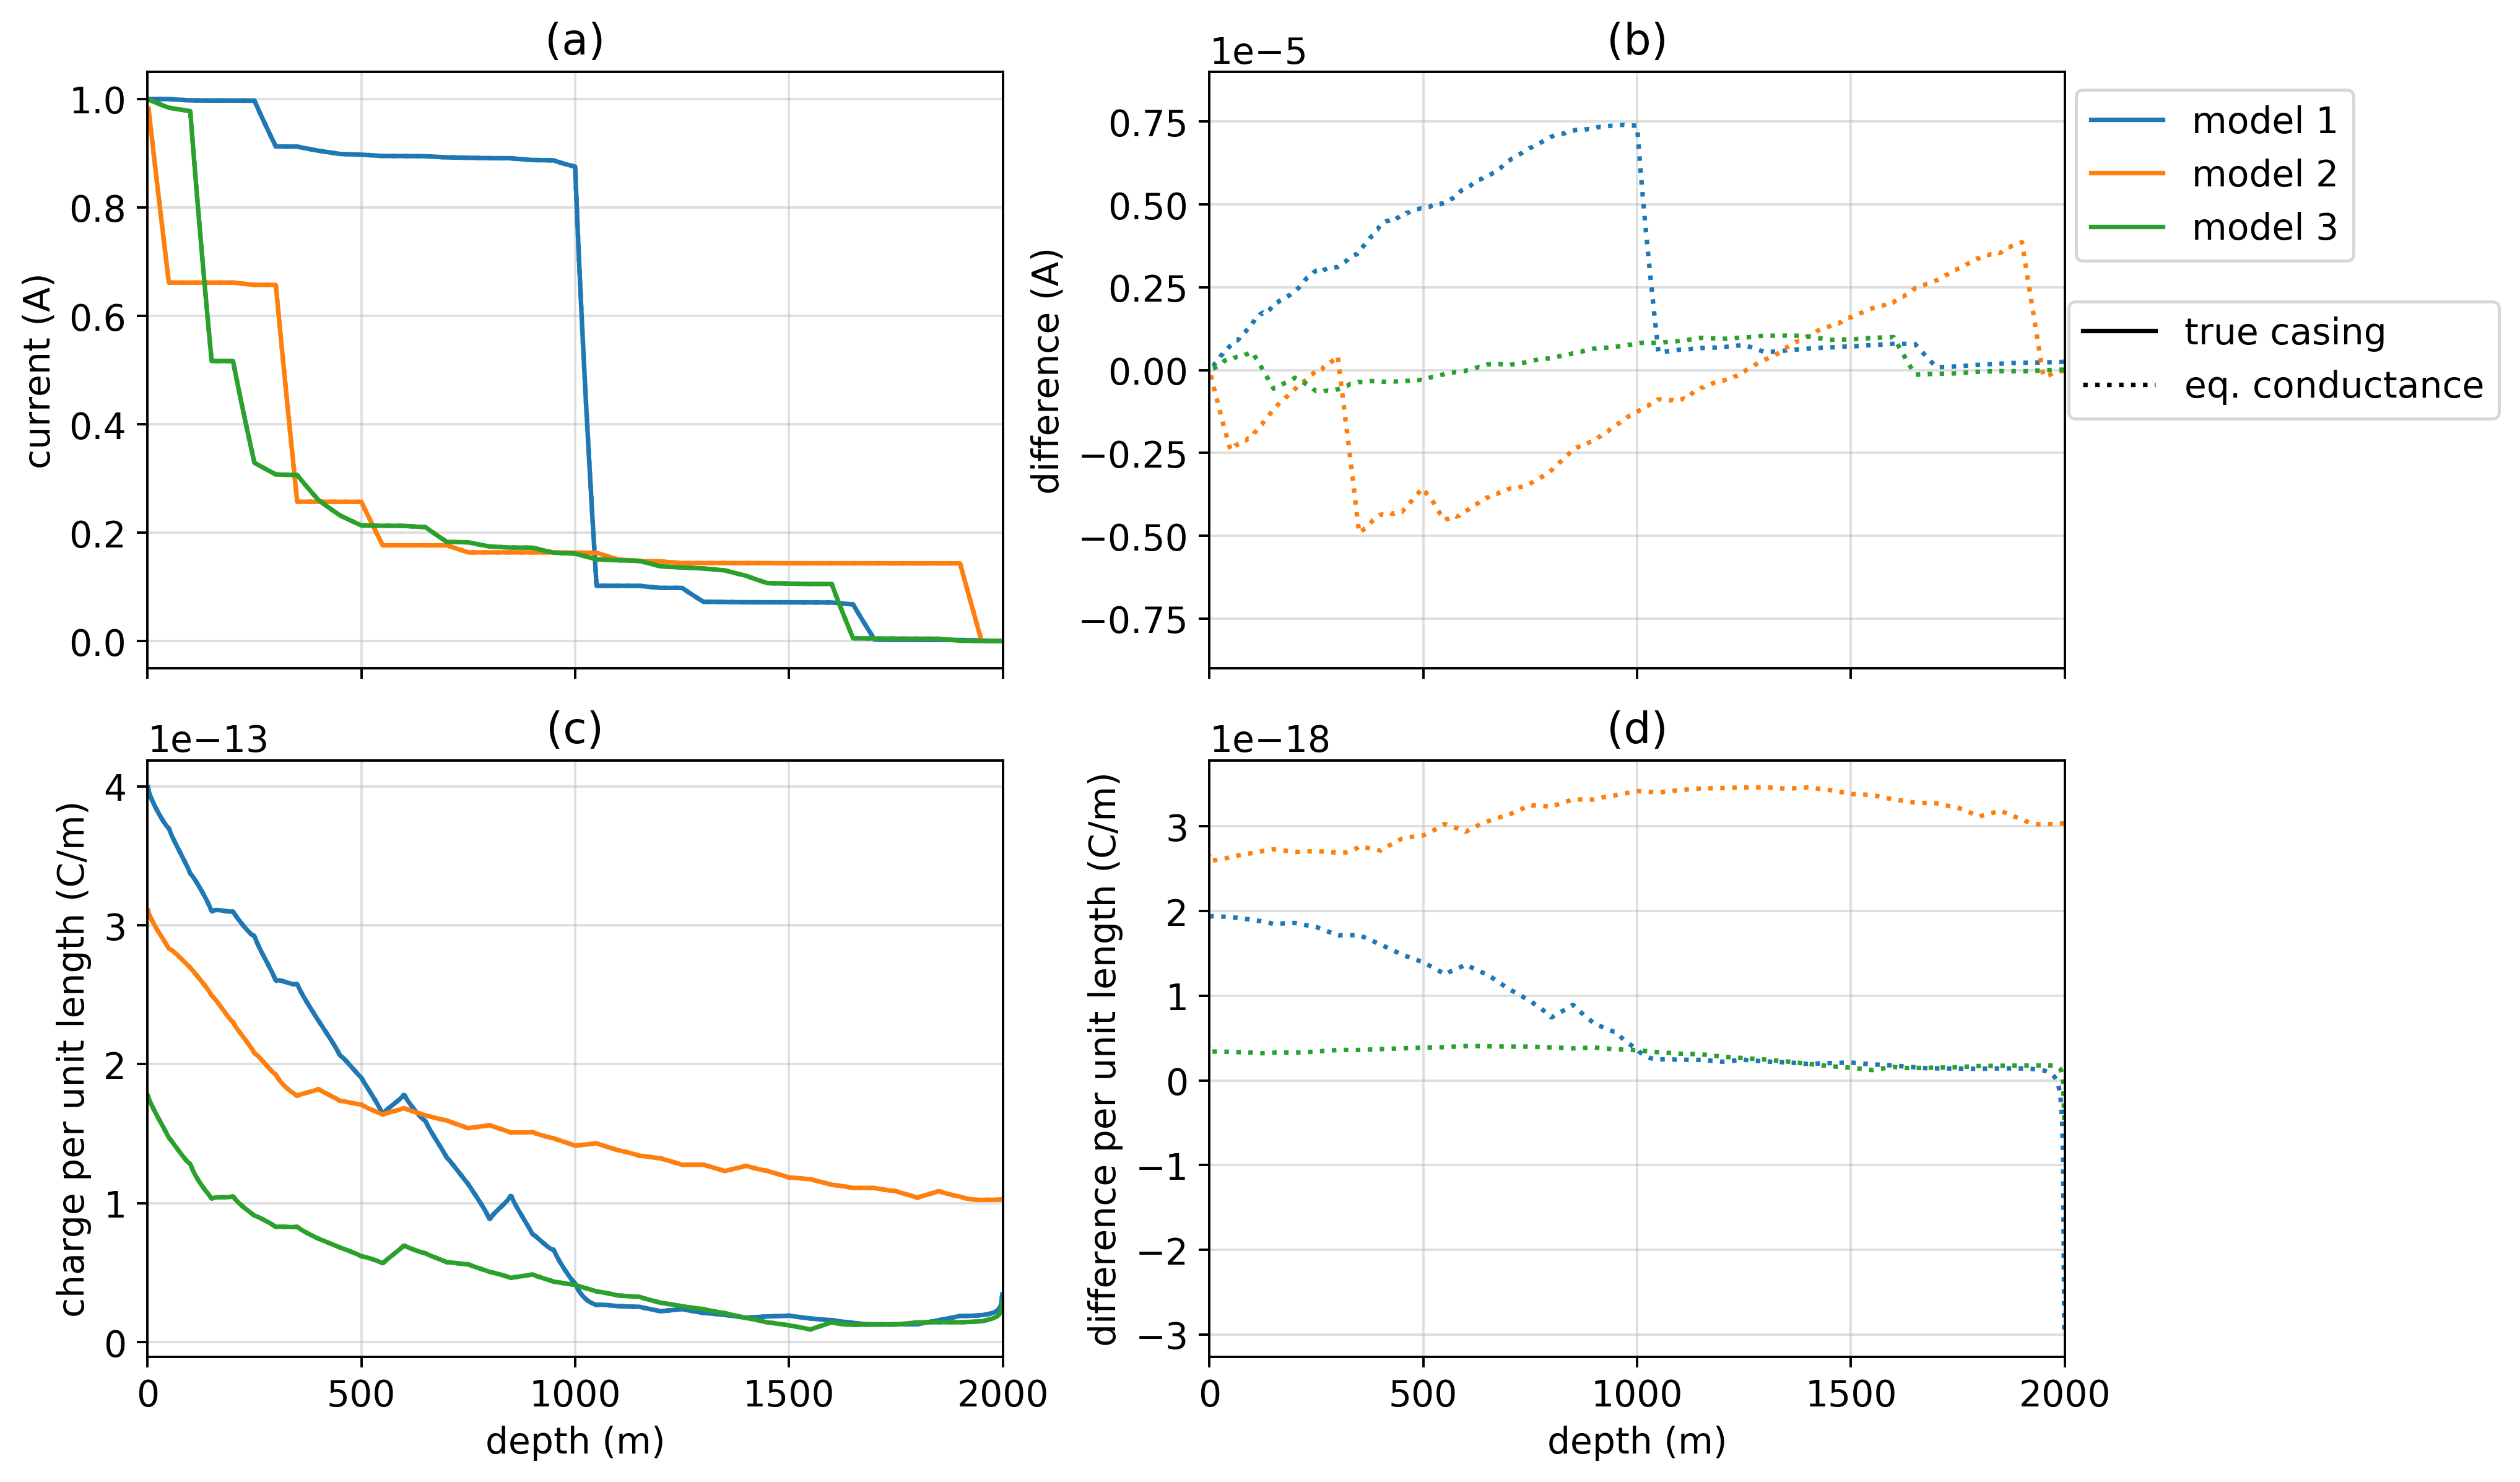
\includegraphics[width=\textwidth]{figures/approximating_wells_currents_charges_random.png}
    \end{center}
\caption{
    (a) Total vertical current through the casing for the three layered-earth models shown in
    Figure \ref{fig:random_layers}. The solid lines indicate the response of the true, hollow steel cased-well
    and the dotted lines indicate the response of a solid cylinder having the same cross-sectional conductance
    as the hollow well. (b) Difference between the currents along the casing in the solid well approximation
    and the true, hollow well.
    (c) Charge per unit length for each of the models. (d) Difference in charge per unit length between the
    true model of the casing and the approximation which preserves cross-sectional conductance.
}
\label{fig:approximating_wells_currents_charges_random}
\end{figure}
